\documentclass[conference]{IEEEtran}
\IEEEoverridecommandlockouts

\usepackage{cite}
\usepackage{amsmath,amssymb,amsfonts}
\usepackage{algorithmic}
\usepackage{graphicx}
\usepackage{textcomp}
\usepackage{xcolor}
\usepackage{booktabs}
\usepackage{array}
\usepackage{url}
\usepackage[hidelinks]{hyperref}

\def\BibTeX{{\rm B\kern-.05em{\sc i\kern-.025em b}\kern-.08em
    T\kern-.1667em\lower.7ex\hbox{E}\kern-.125emX}}

\begin{document}

\title{Deliberation or Diversity? A Controlled Study of\\
Multi-Agent AI Feedback for Direct Preference\\
Optimization of Small Language Models}

\author{\IEEEauthorblockN{Dhruv Singhal}
\IEEEauthorblockA{\textit{Dept. of Computer Science and Engineering} \\
\textit{RV College of Engineering (RVCE)}\\
Bengaluru, India \\
USN: 1RV24CS077 \\
dhruv.singhal1605@gmail.com}}

\maketitle

\begin{abstract}
Direct Preference Optimization (DPO) has become the dominant, compute-efficient
alternative to reinforcement-learning-based alignment, but it still depends on
preference pairs whose collection from human annotators is the single most
expensive stage of the alignment pipeline. Reinforcement Learning from AI
Feedback (RLAIF) replaces those human labels with model-generated ones, yet it
remains unclear \emph{which} ingredient of a modern multi-agent labelling
pipeline actually drives downstream quality. We present the design and reference
implementation of a controlled study that isolates two candidate mechanisms:
\textit{candidate diversity} (several personas answering a prompt) and
\textit{deliberation} (a panel of heterogeneous judges debating over two rounds),
measured at matched inference compute through a $2{\times}2$ factorial design.
Every preference set is used to train an identical Qwen2.5-1.5B-Instruct policy
with the same LoRA/QLoRA DPO recipe, so the \emph{source of the labels} is the
only variable. We further propose \emph{disagreement-aware DPO}, which converts
inter-judge disagreement into a per-pair label-smoothing term. Evaluation uses a
length-controlled win-rate adjudicated by an independent jury of model families
that never participated in labelling, alongside rule-checked capability
benchmarks, with paired-bootstrap confidence intervals and Holm correction. The
entire framework is engineered to run at zero marginal cost on free-tier APIs and
a single Google Colab T4 GPU. We describe the architecture, the labelling and
evaluation protocols and the reproducibility design, and report two early
measurements on human-labelled data: an interpretable reward-model analysis of
what HH-RLHF annotators reward, and a 50-pair check of how often the judge panel
agrees with human labels.
\end{abstract}

\begin{IEEEkeywords}
preference optimization, RLAIF, multi-agent systems, LLM-as-a-judge, direct
preference optimization, parameter-efficient fine-tuning, model alignment
\end{IEEEkeywords}

\section{Introduction}
Reinforcement Learning from Human Feedback (RLHF)~\cite{ouyang2022instructgpt}
and its simpler successor, Direct Preference Optimization
(DPO)~\cite{rafailov2023dpo}, are the dominant techniques for aligning language
models with human preferences. Both consume \emph{preference pairs}: a prompt, a
``chosen'' response, and a ``rejected'' response. Gathering these pairs from
human annotators is the costliest part of the alignment pipeline---the reason the
HH-RLHF corpus~\cite{bai2022hh} required large-scale paid annotation.

Reinforcement Learning from AI Feedback
(RLAIF)~\cite{bai2022constitutional,lee2023rlaif} replaces human labels with
model-generated ones and has been shown to be competitive with human feedback on
several tasks. In parallel, a rich toolbox of multi-agent methods---persona
ensembles, multi-agent debate~\cite{du2023debate}, and LLM-as-a-judge
scoring~\cite{zheng2023judge}---has emerged for eliciting higher-quality signals
from language models. These components are frequently \emph{combined} in modern
labelling stacks, but their contributions are rarely separated: when a
multi-agent pipeline outperforms a single-model baseline, it is seldom clear
whether the gain comes from generating a \emph{more diverse} set of candidate
answers or from a \emph{more deliberative} judging procedure, and whether either
survives once inference compute is held constant.

This paper presents the design and open reference implementation of a controlled
study built to answer that question for the practically important regime of
\emph{small} language models aligned under a strict zero-cost budget. Our guiding
research questions are:
\begin{enumerate}
\item \textbf{Label quality.} How accurately do agent-generated preference labels
match human labels (HH-RLHF) and verifiable ground truth (GSM8K), and what biases
(length, position) do they carry?
\item \textbf{Mechanism.} Is the benefit of a multi-agent pipeline driven by
candidate diversity or by deliberation, at matched compute?
\item \textbf{Downstream effect.} How does DPO on agent labels compare with DPO on
human labels across model families, sizes, and data scales?
\item \textbf{Method.} Does treating panel disagreement as per-pair label
uncertainty (disagreement-aware DPO) narrow the gap to human labels?
\end{enumerate}

\noindent\textbf{Contributions.}
(i) A $2{\times}2$ factorial design that cleanly separates \emph{diversity} from
\emph{deliberation} in AI feedback at matched inference compute, embedded in a set
of reference and adversarial baselines (human, random, longest-answer,
self-consistency);
(ii) \emph{disagreement-aware DPO}, a minimal modification that propagates
inter-judge disagreement into the DPO loss as a per-pair label-smoothing term;
(iii) an evaluation protocol with an enforced judge-independence rule and a
length-controlled win-rate that prevents the most common confounds in
LLM-as-a-judge evaluation; and
(iv) a fully configuration-driven, resumable, cache-backed implementation that
reproduces the entire study at \$0 marginal cost on free-tier infrastructure.

\section{Background and Related Work}

\subsection{From RLHF to DPO}
Classic RLHF~\cite{ouyang2022instructgpt} trains a separate reward model on
preference pairs and then optimizes the policy against it with reinforcement
learning (typically PPO). This is compute-heavy and unstable to tune. DPO
reframes the same objective as a single closed-form, classification-style loss on
the policy's log-probabilities of the chosen versus rejected response, removing
the reward model and the RL loop~\cite{rafailov2023dpo}. The stability and low
cost of DPO are precisely what make preference optimization viable on a single
free GPU, where PPO-based RLHF would not be.

\subsection{Parameter-Efficient Fine-Tuning}
Low-Rank Adaptation (LoRA)~\cite{hu2021lora} freezes the base weights and trains
small rank-decomposed adapters injected into the projection layers, cutting
trainable parameters and memory by an order of magnitude. QLoRA~\cite{dettmers2023qlora}
adds 4-bit quantization of the frozen base, so even multi-billion-parameter models
fit on a single 16\,GB GPU. For the 0.5--3.8B policies studied here, LoRA/QLoRA is
what makes DPO feasible on free-tier hardware.

\subsection{AI Feedback and Multi-Agent Methods}
Constitutional AI~\cite{bai2022constitutional} popularized using AI feedback in
place of human feedback for harmlessness, and a direct empirical comparison of
AI- versus human-generated labels was reported as RLAIF~\cite{lee2023rlaif}.
Multi-agent debate improves factuality and reasoning by having models critique and
revise each other's answers~\cite{du2023debate}, while LLM-as-a-judge studies
document systematic biases---verbosity, position, and self-preference---that any
AI-feedback pipeline must control for~\cite{zheng2023judge}. The individual
pieces are established; the contribution here is a \emph{controlled ablation} in
which the base model, DPO recipe, and evaluation harness are held fixed and the
only variable is the source and construction of the preference labels.

\section{Problem Formulation}
Let $\pi_\theta$ be the policy initialized from a reference model $\pi_{\text{ref}}$,
and let $\mathcal{D}=\{(x, y_w, y_l)\}$ be a set of preference triples with prompt
$x$, chosen response $y_w$, and rejected response $y_l$. DPO minimizes
\begin{equation}
\mathcal{L}_{\text{DPO}}
= -\,\mathbb{E}_{(x,y_w,y_l)\sim\mathcal{D}}
\Big[\log \sigma\big(\beta\, \Delta(x,y_w,y_l)\big)\Big],
\label{eq:dpo}
\end{equation}
\begin{equation}
\Delta(x,y_w,y_l)=
\log\frac{\pi_\theta(y_w\mid x)}{\pi_{\text{ref}}(y_w\mid x)}
-\log\frac{\pi_\theta(y_l\mid x)}{\pi_{\text{ref}}(y_l\mid x)},
\end{equation}
where $\sigma$ is the logistic function and $\beta$ controls the deviation from
$\pi_{\text{ref}}$. Under parameter-efficient training, $\pi_{\text{ref}}$ is the
same base network with the LoRA adapter disabled, so no second model need be
loaded.

The study holds $\pi_\theta$, $\pi_{\text{ref}}$, $\beta$, and the optimization
schedule fixed across all conditions. The experimental variable is the
\emph{construction of $\mathcal{D}$}: whether candidates come from one persona or
several, whether the chosen/rejected decision is made by a single self-consistent
judge or a deliberating panel, and whether the human-labeled HH-RLHF pairs are
substituted as a gold-standard reference.

\section{System Architecture}
The system is split into two layers that are kept conceptually and operationally
separate (Fig.~\ref{fig:arch}). \textbf{Layer~A} (data generation) is agentic and
prompt-engineering only---it never touches model weights and performs only LLM API
calls. \textbf{Layer~B} (training and evaluation) is the machine-learning core:
LoRA adapters, the DPO loss, and a held-out evaluation harness. Every parameter of
both layers lives in version-controlled YAML configuration files; no experimental
constant is hard-coded, and each run writes a snapshot of its fully resolved
configuration for provenance.

\begin{figure}[t]
\centering
\setlength{\fboxsep}{6pt}
\framebox[0.95\columnwidth]{%
\begin{minipage}{0.88\columnwidth}
\footnotesize
\textbf{Layer A --- Data generation (free-tier APIs)}\\[2pt]
Seed prompt $x$ \;$\rightarrow$\; \{persona$_1$ \dots persona$_k$\} generate
$n{=}4$ candidates \;$\rightarrow$\; judge (self-consistency \emph{or} debating
panel) \;$\rightarrow$\; $(x, y_w, y_l)$ + agreement score.\\[6pt]
\hrule
\vspace{4pt}
\textbf{Layer B --- Training \& evaluation (single T4 GPU)}\\[2pt]
Preference set $\mathcal{D}$ \;$\rightarrow$\; LoRA/QLoRA DPO on fixed policy
\;$\rightarrow$\; length-controlled win-rate (independent jury) + capability
benchmarks + paired-bootstrap CIs.
\end{minipage}}
\caption{Two-layer architecture. The boundary between agentic data generation and
the ML training core is strict: the only thing that changes between experimental
conditions is the preference set produced by Layer~A.}
\label{fig:arch}
\end{figure}

\subsection{Base Model Selection}
The policy must (a) run on a free 16\,GB T4 with LoRA, (b) carry a permissive
license, (c) follow instructions well enough that DPO refines rather than teaches
behavior, and (d) be well supported by the Hugging Face \texttt{transformers},
\texttt{trl}, \texttt{peft}, and Unsloth stack. Table~\ref{tab:models} summarizes
the candidates considered. We adopt \textbf{Qwen2.5-1.5B-Instruct}
(Apache-2.0)~\cite{qwen25} as the primary policy for its balance of capability,
license, and training speed, and use Qwen2.5-0.5B-Instruct, SmolLM3-3B, and
Phi-4-mini-instruct---all Apache-2.0 or MIT---as a generalization set spanning
size and model family.

\begin{table}[t]
\caption{Candidate Base Policies (Permissively Licensed Subset)}
\label{tab:models}
\centering
\footnotesize
\begin{tabular}{@{}lll@{}}
\toprule
\textbf{Model} & \textbf{Params} & \textbf{License} \\
\midrule
Qwen2.5-1.5B-Instruct (primary) & 1.5\,B & Apache-2.0 \\
Qwen2.5-0.5B-Instruct & 0.5\,B & Apache-2.0 \\
SmolLM3-3B & 3\,B & Apache-2.0 \\
Phi-4-mini-instruct & 3.8\,B & MIT \\
\bottomrule
\end{tabular}
\end{table}

\section{The Multi-Agent Labelling Pipeline}
Layer~A turns each seed prompt into one preference pair plus a scalar agreement
score. It has two factors, corresponding directly to the two hypothesized
mechanisms.

\subsection{Factor 1 --- Candidate Diversity}
For every prompt the generator produces $n=4$ candidate answers at temperature
$0.8$. In the \emph{single-persona} level all four share one neutral
helpful-assistant system prompt, so their diversity comes only from sampling
noise. In the \emph{multi-persona} level the four answers come from four distinct
personas---concise, step-by-step, domain-expert, and careful-skeptic---each of
which nonetheless begins from the same helpful-assistant instruction so that
personas vary \emph{style and depth}, not \emph{willingness to help}. A shared
length instruction (``keep your answer under 200 words'') is appended to every
persona in both levels, so answer length is never a hidden difference between
conditions.

\subsection{Factor 2 --- Deliberation}
A judge converts the candidate set into a chosen/rejected ordering against a fixed
rubric scoring \emph{helpfulness}, \emph{correctness}, and \emph{harmlessness} on a
$1$--$5$ scale. The rubric explicitly instructs judges to score substance rather
than length or style; length bias is nonetheless \emph{measured} afterward rather
than assumed away. Candidates are shown in a freshly randomized order on every
call, and the permutation is logged, so position bias averages out. The two levels
of this factor are matched at exactly six model calls per prompt:
\begin{itemize}
\item \textbf{Single judge (self-consistency).} One strong judge model scores the
candidates in six independent samples; all six are treated as final verdicts.
\item \textbf{Panel (deliberation).} Three judges from two model families score
independently in round~1, then in round~2 each judge sees the others' round-1
rationales and may revise~\cite{du2023debate}. Three judges $\times$ two rounds
$=$ six calls; only the three round-2 verdicts are final.
\end{itemize}
Each candidate's score is the mean over rubric criteria; the chosen answer is the
one with the highest mean over final verdicts and the rejected answer the lowest,
with exact ties broken by a seeded coin flip rather than by candidate order. The
aggregation rule is identical across both judging levels so it cannot act as a
hidden third difference. For every pair, the fraction of final verdicts that agree
on the chosen-over-rejected ordering is recorded as an agreement score in
$\{1/3,\dots,1\}$.

\subsection{Robustness and Cost Engineering}
Verdicts are returned as JSON validated with a typed schema and retried on parse
failure. Every API request---keyed by model, messages, parameters, and sample
index---is hashed and cached in SQLite, so re-running never re-spends free-tier
quota and the exact raw outputs behind the dataset are preserved. Requests use
exponential backoff with jitter on rate-limit and server errors, and every stage
is resumable: a prompt that fails after retries is simply absent from its output
file and is picked up on the next run. A dry-run budgeting command reports the
per-model API calls and days required for any plan before a single token is spent.

\section{Experimental Design}
The core of the study is a set of conditions that share everything except the
preference labels (Table~\ref{tab:conditions}).

\begin{table}[t]
\caption{Experimental Conditions}
\label{tab:conditions}
\centering
\footnotesize
\begin{tabular}{@{}lll@{}}
\toprule
\textbf{Condition} & \textbf{Candidates} & \textbf{Labels} \\
\midrule
\multicolumn{3}{@{}l}{\textit{References and baselines}}\\
\texttt{base}        & ---            & untuned (zero point) \\
\texttt{human}       & HH-RLHF        & human (gold standard) \\
\texttt{random}      & multi-persona  & coin flip (floor) \\
\texttt{length}      & multi-persona  & longer answer \\
\midrule
\multicolumn{3}{@{}l}{\textit{The $2{\times}2$ factorial (6 judge calls each)}}\\
\texttt{single\_single} & single persona & single judge \\
\texttt{single\_panel}  & single persona & panel \\
\texttt{multi\_single}  & multi-persona  & single judge \\
\texttt{multi\_panel}   & multi-persona  & panel \\
\midrule
\multicolumn{3}{@{}l}{\textit{Method and variants}}\\
\texttt{multi\_panel\_da} & multi-persona & panel + disagree.-aware \\
\texttt{onpolicy\_panel}  & policy samples & panel \\
\bottomrule
\end{tabular}
\end{table}

The $2{\times}2$ interior (\texttt{single\_single}, \texttt{single\_panel},
\texttt{multi\_single}, \texttt{multi\_panel}) is the mechanism experiment:
diversity on/off crossed with deliberation on/off, all at six judge calls per
prompt. \texttt{single\_single} is the plain-RLAIF baseline;
\texttt{multi\_panel} is the full pipeline. The \texttt{random} and
\texttt{length} conditions are adversarial baselines: if coin-flip labels train as
well as agent labels there is no signal, and if ``pick the longer answer'' matches
the agents, the agent signal is mostly a length preference---something worth
knowing before reviewers raise it. An \texttt{onpolicy\_panel} variant draws
candidates from the policy's own distribution, which often trains better than
answers written by a much larger model~\cite{tajwar2024onpolicy}.

The main grid uses 1{,}000 pairs per condition with three training seeds; a
generalization sweep repeats the headline conditions on three further models; and
a scaling curve (250/500/1000/2000 pairs, with nested subsets so larger sets
strictly contain smaller ones) tests whether the agent--human gap shrinks with
scale. All hyperparameters are frozen \emph{once} by a pilot sweep run jointly on
the human and full-agent datasets, so tuning never silently favors one condition.

\subsection{Disagreement-Aware DPO}
Panel disagreement is a natural, free estimate of label noise: pairs on which the
judges split are more likely mislabeled. We propose replacing the constant DPO
label-smoothing term with a per-pair value derived from the recorded agreement.
Writing $a_i\in\{1/3,\dots,1\}$ for the agreement on pair $i$, the conditional DPO
(cDPO) objective
\begin{equation}
\mathcal{L}_i = -(1-\epsilon_i)\log\sigma(\beta\Delta_i)
               - \epsilon_i\,\log\sigma(-\beta\Delta_i)
\label{eq:cdpo}
\end{equation}
uses $\epsilon_i = \epsilon_{\max}(1-a_i)$, so unanimous pairs are trusted fully
($\epsilon_i\!\to\!0$) while contested pairs are down-weighted toward a uniform
target. This requires no extra labels or compute beyond the agreement score the
panel already produces. Equation~\eqref{eq:cdpo} defines the method evaluated in
the \texttt{multi\_panel\_da} condition; the current reference implementation
flags it explicitly as not yet wired into the trainer, and realizing it is the
immediate next step (Section~\ref{sec:status}).

\subsection{Datasets}
Seed prompts are drawn from the HH-RLHF helpful-base and harmless-base subsets,
stratified 50/50 and restricted to single-turn prompts of 4--256 policy tokens.
The same prompts' real human-labeled pairs form the \texttt{human} reference.
Exact and near-duplicate prompts (cosine similarity $\geq 0.90$ over MiniLM
embeddings) are removed so training prompts cannot leak into evaluation. GSM8K
supplies a verifiable domain in which a candidate's final answer can be checked
against gold, giving an objective label-accuracy measurement independent of any
judge.

\section{Evaluation Protocol}
\label{sec:eval}
Every model---including the untuned base---passes through an identical harness with
greedy decoding on the same held-out prompts.

\subsection{Length-Controlled Win-Rate with an Independent Jury}
The headline metric is a pairwise win-rate judged by a jury of model families.
Each pair is judged twice with the A/B positions swapped; disagreement between the
two orders is counted as a tie, removing position bias rather than averaging over
it. A strict majority of jurors is required for a win. Crucially, a
\textbf{judge-independence rule} is enforced in code: no evaluation juror may share
a model family with (a) the policy being evaluated---which would invite
self-preference~\cite{zheng2023judge}---or (b) any model used to generate or label
the training data, since the policy was trained on that judge's taste and would be
grading its own homework. Two independent families (Gemini and Cohere) serve as
jurors. Because LLM judges favor longer answers, we additionally report a
length-controlled win-rate in the style of AlpacaEval~2~\cite{dubois2024alpaca}: a
logistic regression of the verdict on the length difference, read off at zero
length difference, reported beside the raw rate so length cannot inflate the
headline number.

\subsection{Capability Retention and Statistics}
To check that alignment does not degrade core ability, we run IFEval,
TruthfulQA-MC2, GSM8K, and MMLU through the EleutherAI
\texttt{lm-evaluation-harness} for standard, comparable scoring; the rule- and
log-prob-checked tasks need no judge. Uncertainty is quantified with a paired
bootstrap over prompts (10{,}000 resamples): because every model answers the same
prompts, resampling prompts rather than individual answers yields honest
confidence intervals for \emph{differences} between models. Results are averaged
over three seeds with the seed-to-seed standard deviation reported, and because
many conditions are compared, $p$-values are Holm-corrected to hold the
family-wise error rate at 5\%.

\section{Implementation and Reproducibility}
The framework is a Python package organized as a thin numbered-script CLI over a
library core. Training supports two interchangeable backends resolved
automatically from the hardware: Unsloth-patched 4-bit QLoRA on a CUDA T4, and
plain PEFT LoRA in full precision on Apple MPS or CPU, so the same experiment code
runs on a laptop for development and on a free Colab/Kaggle GPU for the full
study. The LoRA configuration adapts all attention and MLP projections at rank
$16$ ($\alpha=32$), trained for two epochs at learning rate $5\times10^{-6}$ with
an effective batch size of 16 and $\beta=0.1$; adapters (tens of MB) are
checkpointed every 25 steps so an interrupted free session loses at most minutes
of work. Reproducibility is enforced structurally: all randomness is seeded, every
run snapshots its resolved configuration, preference sets are built over the
intersection of prompts valid in all conditions (and locked by a manifest so
changing the condition set cannot silently alter which prompts a model trains on),
and a test suite covers parsing, schema validation, and the statistics without
needing network access or API keys. The upper-bound compute for the full study is
roughly 90 GPU-runs ($\approx$60--80 T4 GPU-hours), all within free-tier limits.

\section{Auxiliary Reward Model and Explainability}
\label{sec:reward}
Before any policy is trained, we ask a cheaper diagnostic question: \emph{which
observable properties of a response predict that it is preferred?} If a label
source can be predicted largely from superficial cues such as length, a policy
trained on it is likely to learn those cues. We therefore fit an interpretable
pairwise reward model to each preference set.

\subsection{Model}
Each response $y$ is mapped to a feature vector $\phi(y)$ comprising five named
text signals---log word count, hedge-phrase count, refusal-phrase count, question
marks, and list items (matched on whole words)---plus the first eight principal
components of a MiniLM sentence embedding. Following the Bradley--Terry
model~\cite{bradley1952}, $P(y_c \succ y_r)=\sigma\!\big(w^{\top}[\phi(y_c)-\phi(y_r)]\big)$
is fitted by L2-regularized logistic regression on standardized feature
differences, with no intercept so that the score is antisymmetric in its two
arguments. Pairwise accuracy is estimated out-of-fold with 5-fold
cross-validation (PCA refitted within each training fold) and reported with a
bootstrap 95\% CI, beside a ``longer response wins'' baseline. Attributions are
computed with linear SHAP~\cite{lundberg2017shap}; for each embedding component,
the responses at its two extremes are inspected so the axis can be named.

\subsection{Results on Human Labels}
Table~\ref{tab:reward} reports the model on 2{,}000 HH-RLHF training pairs.
Pooled over both subsets, the model barely clears the length baseline. Fitted per
subset, however, accuracy rises to 63--67\%, and Fig.~\ref{fig:subset} shows why:
the two subsets reward \emph{opposite} behavior. In \texttt{helpful-base}, longer
answers are preferred and refusals penalized; in \texttt{harmless-base}, shorter
answers and refusals are preferred, and the length baseline falls well
\emph{below} chance (40.6\%). In the pooled model, the strongest single direction
(embedding PC8, coefficient $-0.21$) separates eager compliance (e.g. ``Sure,
here's a list of profanities'') from cautious, deferring answers, and is
penalized; an empathy direction (PC6, ``I'm sorry to hear that\ldots'') is
rewarded. Two implications follow for the main study: AI judges must be checked
separately on helpfulness and harmlessness prompts, since a judge with a single
global length preference would agree with humans on one subset and disagree on
the other; and the length-controlled win-rate of Section~\ref{sec:eval} is
warranted, since length is a first-order preference signal in this data.

\begin{table}[t]
\caption{Pairwise reward model on HH-RLHF human labels (5-fold CV). Len.\ base: accuracy of ``the longer response wins''.}
\label{tab:reward}
\centering
\begin{tabular}{@{}lrcc@{}}
\toprule
Pairs & $n$ & Acc.\ [95\% CI] & Len.\ base \\
\midrule
All, text only & 2000 & 52.7\% [50.5, 54.8] & 51.8\% \\
All, text + PCs & 2000 & 56.5\% [54.3, 58.7] & 51.8\% \\
\texttt{helpful-base}    & 1000 & 67.2\% [64.3, 70.1] & 63.0\% \\
\texttt{harmless-base}   & 1000 & 62.9\% [60.0, 65.8] & 40.6\% \\
\bottomrule
\end{tabular}
\end{table}

\begin{figure}[t]
\centering
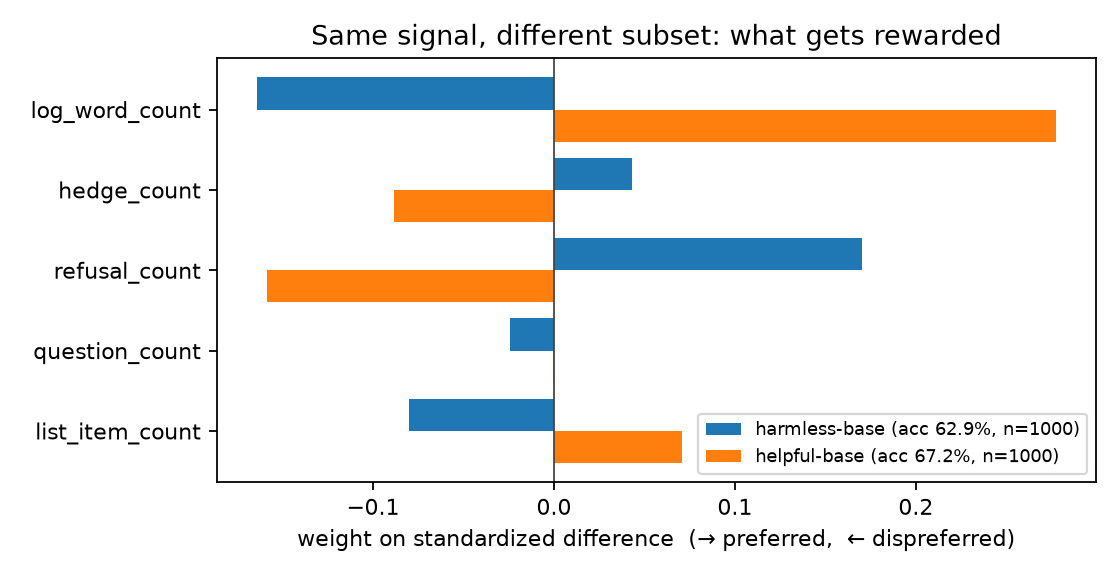
\includegraphics[width=\columnwidth]{figures/subset_coefficients.png}
\caption{Standardized reward-model weights on the five named text features, fitted
separately per HH-RLHF subset. Length and refusals flip sign between subsets.}
\label{fig:subset}
\end{figure}

\section{Pilot and Current Status}
\label{sec:status}
A reduced-scale ``demo'' profile runs the same code, prompts, judges, and DPO loss
as the full study with a 0.5B policy, 150 pairs, and the \texttt{base},
\texttt{human}, and \texttt{multi\_panel} conditions. So far it has been run
only in part: candidate generation and panel judging for 22 training prompts
(yielding 15 preference pairs; the others produced no usable pair) and greedy
generation of the base policy's responses to 100 evaluation prompts. DPO training
and the win-rate evaluation have not yet been run, so we report no policy-level
results.

\textbf{Label-agreement pilot.} As a first label-quality check, the panel judged
50 held-out HH-RLHF pairs from the \texttt{label\_agreement} split, shown in
shuffled order, and we compared its choice with the human label (a panel tie
counts as half). The panel agreed with the human label on 68.0\% of pairs
(bootstrap 95\% CI 56--80\%; 69.6\% on \texttt{harmless-base}, 66.7\% on
\texttt{helpful-base}). Agreement was strongly tied to panel consensus:
80.6\% when the final verdicts were unanimous ($n{=}31$) against 46.2\%, no
better than chance, when they were split ($n{=}13$); six pairs were scored as
ties. This is the pattern disagreement-aware DPO is designed to exploit:
inter-judge disagreement flags the labels least likely to be right. Judges named
the first-shown response best in 48.7\% of 300 calls, so the shuffling leaves no
detectable position bias. Deliberation changed individual judges' agreement
only modestly (round 1 $\rightarrow$ round 2: $70\rightarrow74\%$,
$70\rightarrow68\%$, $64\rightarrow66\%$). With $n{=}50$ these are pilot
estimates; the full check uses all 500 pairs. A qualitative inspection of pilot
agent pairs also shows the limit of consensus: for a factual lookup prompt, all
four candidates gave fabricated addresses and the panel unanimously rated one
of them 5/5, which motivates the GSM8K check against gold answers.

Two items remain before the full grid: wiring the disagreement-aware
loss of Eq.~\eqref{eq:cdpo} into the trainer, and executing the main grid,
generalization sweep, and scaling curve on free GPU time. This paper documents the
design and reference implementation so that the subsequent empirical results are
interpretable and reproducible.

\section{Threats to Validity}
\textbf{Construct validity.} LLM-judge win-rate is a proxy for human preference;
we mitigate its known failure modes through the judge-independence rule, position
swapping, and length control, but it cannot fully substitute for a human study.
\textbf{Internal validity.} Matching the two factors at six calls per prompt
controls for raw compute, yet ``one strong judge sampled six times'' and ``three
judges over two rounds'' still differ in model identity; the single-judge and
panel pools are chosen from the same free catalogue to keep this gap small.
\textbf{External validity.} Findings are scoped to small (0.5--3.8B) instruction-tuned
policies and to the free model catalogue available at the time of the runs, which
changes frequently; the generalization sweep across families and sizes is intended
to probe how far conclusions travel. \textbf{Data validity.} HH-RLHF prompts and
the free judge models carry their own biases; GSM8K provides an independent,
verifiable cross-check on label accuracy.

\section{Conclusion}
We have presented the design and open reference implementation of a controlled
study that asks not merely \emph{whether} multi-agent AI feedback helps DPO on
small language models, but \emph{why}---separating candidate diversity from
deliberation at matched compute, anchoring both against human, random, and
length baselines, and proposing a disagreement-aware DPO loss that recycles panel
disagreement as free label-uncertainty information. The framework is engineered
end to end for zero-cost reproducibility on free-tier infrastructure, with an
evaluation protocol hardened against the standard confounds of LLM-as-a-judge
measurement. Completing the empirical grid---and determining which of diversity or
deliberation, if either, is the operative mechanism---is the direct next step.

\begin{thebibliography}{00}
\bibitem{ouyang2022instructgpt} L. Ouyang \textit{et al.}, ``Training language
models to follow instructions with human feedback,'' in \textit{Proc. NeurIPS},
2022.
\bibitem{rafailov2023dpo} R. Rafailov, A. Sharma, E. Mitchell, S. Ermon, C. D.
Manning, and C. Finn, ``Direct preference optimization: Your language model is
secretly a reward model,'' in \textit{Proc. NeurIPS}, 2023.
\bibitem{bai2022hh} Y. Bai \textit{et al.}, ``Training a helpful and harmless
assistant with reinforcement learning from human feedback,'' \textit{arXiv
preprint arXiv:2204.05862}, 2022.
\bibitem{bai2022constitutional} Y. Bai \textit{et al.}, ``Constitutional AI:
Harmlessness from AI feedback,'' \textit{arXiv preprint arXiv:2212.08073}, 2022.
\bibitem{lee2023rlaif} H. Lee \textit{et al.}, ``RLAIF vs. RLHF: Scaling
reinforcement learning from human feedback with AI feedback,'' \textit{arXiv
preprint arXiv:2309.00267}, 2023.
\bibitem{du2023debate} Y. Du, S. Li, A. Torralba, J. B. Tenenbaum, and I. Mordatch,
``Improving factuality and reasoning in language models through multiagent
debate,'' \textit{arXiv preprint arXiv:2305.14325}, 2023.
\bibitem{zheng2023judge} L. Zheng \textit{et al.}, ``Judging LLM-as-a-judge with
MT-Bench and Chatbot Arena,'' in \textit{Proc. NeurIPS Datasets and Benchmarks},
2023.
\bibitem{hu2021lora} E. J. Hu \textit{et al.}, ``LoRA: Low-rank adaptation of
large language models,'' in \textit{Proc. ICLR}, 2022.
\bibitem{dettmers2023qlora} T. Dettmers, A. Pagnoni, A. Holtzman, and L.
Zettlemoyer, ``QLoRA: Efficient finetuning of quantized LLMs,'' in \textit{Proc.
NeurIPS}, 2023.
\bibitem{tajwar2024onpolicy} F. Tajwar \textit{et al.}, ``Preference fine-tuning
of LLMs should leverage suboptimal, on-policy data,'' in \textit{Proc. ICML},
2024.
\bibitem{dubois2024alpaca} Y. Dubois, B. Galambosi, P. Liang, and T. B. Hashimoto,
``Length-controlled AlpacaEval: A simple way to debias automatic evaluators,''
\textit{arXiv preprint arXiv:2404.04475}, 2024.
\bibitem{qwen25} Qwen Team, Alibaba, ``Qwen2.5-1.5B-Instruct model card,''
Hugging Face, 2024. [Online]. Available:
\url{https://huggingface.co/Qwen/Qwen2.5-1.5B-Instruct}
\bibitem{bradley1952} R. A. Bradley and M. E. Terry, ``Rank analysis of incomplete
block designs: I. The method of paired comparisons,'' \textit{Biometrika}, vol. 39,
no. 3/4, pp. 324--345, 1952.
\bibitem{lundberg2017shap} S. M. Lundberg and S.-I. Lee, ``A unified approach to
interpreting model predictions,'' in \textit{Proc. NeurIPS}, 2017.
\end{thebibliography}

\end{document}
